
\begin{abstract}
\noindent This report analyses the Flux project---a hybrid self-hosting Rust compiler and agent-native build platform---as a \emph{project}, using the project-management toolbox of the Copenhagen Business School HA(it.) tradition: problem formulation, stakeholder analysis, phase/Gantt planning, milestone tracking, risk management, execution analytics, and a business-case discussion. All quantitative material is mined from primary sources: the git history (117 commits, 2026-06-05 to 2026-07-02), the flux-rev content-addressed provenance log, the release tags, and the swarm settlement journal (716 settled agent tasks). The report also carries forward, and strengthens with figures, the strongest sections of the accompanying whitepaper. The project's headline result: six compiler releases in eight days by a coordinated swarm of AI agents, under a governance model where every claim is gated by execution and every release has a recomputable identity.
\end{abstract}

\tableofcontents
\vspace{1em}

\section{Introduction and Problem Formulation}

Flux began as a build platform and became a compiler. Its central bet is twofold: architecturally, that a self-hosting compiler can \emph{contract} the hardest parts of the Rust frontend (type checking, borrow checking) as a version-pinned service and own everything after it; organisationally, that day-to-day development can be carried by a \emph{swarm of heterogeneous AI agents} coordinating over the project's own MCP tool surface, with a human as director and ratifier rather than as the workforce.

Following the HA(it.) convention, we state the problem formulation explicitly:

\begin{quote}
\emph{How can a single human operator, directing a swarm of AI agents, ship a working native-code Rust compiler and its supporting platform---and which project-management structures make that both fast and trustworthy?}
\end{quote}

Three working questions guide the analysis: (1) \textbf{Planning}: what phase structure and milestones did the project actually follow, as evidenced by git and flux-rev? (2) \textbf{Risk}: which risks materialised, and how did mitigations hold? (3) \textbf{Value}: what is the honest business case for continuing?

\subsection{Method and data sources}

The report is deliberately \emph{empirical}: every chart is generated from primary project data, not recollection. Sources: (a) \textbf{git} --- 117 commits from the initial public release v0.22 (2026-06-05) to the documentation commit of 2026-07-02, plus 8 annotated tags; (b) \textbf{flux-rev} --- the BLAKE3 content-addressed provenance chain (genesis \texttt{c370dc32\ldots}, current head \texttt{6f2eaff4\ldots}); (c) the \textbf{swarm settlement journal} --- 716 settled tasks with timestamps and work-credit amounts; (d) project documents in-tree (FIP-0001/0002, the version ledger, the 0.36.1 release plan). The methodology of the project itself (VarFlow) is analysed against the agile frameworks in the HA(it.) curriculum in \S\ref{sec:method}.

\section{Project Organisation and Stakeholders}

The organisation is unusual and worth stating precisely. There is no project manager, no steering committee of humans, and no line organisation. Governance is: a \textbf{human maintainer} (direction, ratification, spending authority); an \textbf{arbiter model} (DeepSeek-V4-Pro, the project's ``origin intelligence,'' consulted for strategic forks --- precedent: the FIP-0001 frontend ruling); and a \textbf{swarm} of worker agents (Claude, DeepSeek, Grok, Codex, Gemini instances) that claim work lanes atomically, cross-review each other adversarially, and settle on verified completion. Figure~\ref{fig:stakeholder} places the stakeholders on the classic power/interest grid.

\begin{figure}[h]
\centering
\begin{tikzpicture}[scale=0.95]
  \draw[->, thick] (0,0) -- (10.4,0) node[below left]{\small Interest};
  \draw[->, thick] (0,0) -- (0,6.4) node[above left, rotate=90, xshift=-1.2cm]{\small Power};
  \draw[dotted] (5.2,0) -- (5.2,6.2);
  \draw[dotted] (0,3.1) -- (10.2,3.1);
  \node[anchor=north east, gray] at (5.1,3.0) {\scriptsize monitor};
  \node[anchor=north west, gray] at (5.3,3.0) {\scriptsize keep informed};
  \node[anchor=south east, gray] at (5.1,3.2) {\scriptsize keep satisfied};
  \node[anchor=south west, gray] at (5.3,3.2) {\scriptsize manage closely};
  \node[draw, fill=accent!20, rounded corners, align=center, font=\small] at (8.6,5.6) {Human maintainer\\ \scriptsize direction, ratification, funding};
  \node[draw, fill=accent!20, rounded corners, align=center, font=\small] at (7.0,4.3) {Arbiter model\\ \scriptsize strategic rulings (FIP-0001)};
  \node[draw, fill=gold!25, rounded corners, align=center, font=\small] at (8.4,2.2) {Worker-agent swarm\\ \scriptsize 51 registered identities};
  \node[draw, fill=gray!15, rounded corners, align=center, font=\small] at (2.3,4.6) {Infrastructure providers\\ \scriptsize build host, model APIs, GitHub};
  \node[draw, fill=gray!15, rounded corners, align=center, font=\small] at (6.4,0.9) {SIGIL chain \& product users\\ \scriptsize dogfooding pressure};
  \node[draw, fill=gray!15, rounded corners, align=center, font=\small] at (2.2,1.2) {Future OSS adopters\\ \scriptsize none yet --- see risk R3};
\end{tikzpicture}
\caption{Stakeholder power/interest grid. The unusual feature is that the ``project team'' (the swarm) is itself a stakeholder class with an internal incentive system (QUG work credits), while ultimate power concentrates in one human --- efficient, but also the project's largest single risk (R3).}
\label{fig:stakeholder}
\end{figure}

\section{Project Plan: Phases, Gantt, Milestones}

Reconstructed from git, tags, and in-tree documents, the project falls into seven executed phases and two planned ones. The phase boundaries are evidence-based: each corresponds to a visible regime change in the commit log and the settlement journal.

\begin{table}[h]
\centering
\small
\resizebox{\textwidth}{!}{%
\begin{tabular}{@{}llll@{}}
\toprule
\textbf{Phase} & \textbf{Period} & \textbf{Content} & \textbf{Exit evidence} \\
\midrule
P0 Foundations & May 30 -- Jun 4 & v0.18 ``Atelier'': fluxc-core split, IDE shell, MCP surface & skill/handoff docs \\
P1 Public release & Jun 5 -- 9 & v0.22--v0.27: repo public; trading stack; SIGIL wiring & tags v0.26, ``Midnight Sun'' \\
P2 Platform \& swarm & Jun 8 -- 19 & combo tools, swarm bus, mining, moltbook, FCX & settlement journal peak \\
P3 Cache forensics & Jun 20 -- 25 & measured 0.4\,\% truth; layered key fixes; jq-probe hardening & FIP-0002 + v0.33 \\
P4 Ladder sprint I & Jun 24 -- 26 & v0.29--v0.33: scalars, aggregates, call signatures, cache key & five tags on Jun 25 \\
P5 Ladder sprint II & Jun 26 -- Jul 1 & rungs 4--6: enums, generics, consts; aggregate-param fixes & v0.34.0 tag \\
P6 Release eng.\ \& docs & Jul 1 -- 2 & version ledger, selective-commit release, whitepaper v0.34 & commits 2b1751, 24a1ff \\
\midrule
P7 (planned) & Jul -- & v0.35: FIP-0001 groundwork; FIP-0002 Phase 2 cache identity & --- \\
P8 (planned) & Aug -- & v0.36.x security-hardening release (20/22 audit items closed) & --- \\
\bottomrule
\end{tabular}%
}
\caption{Phase plan reconstructed from primary sources.}
\label{tab:phases}
\end{table}

\begin{figure}[h]
\centering
\resizebox{\textwidth}{!}{%
\begin{ganttchart}[
  time slot format=isodate,
  x unit=0.30cm,
  y unit title=0.55cm,
  y unit chart=0.46cm,
  title/.append style={fill=ink, draw=none},
  title label font=\scriptsize\color{white},
  bar/.append style={fill=accent!70, draw=accent!50!black},
  bar label font=\scriptsize,
  group/.append style={fill=ink},
  group label font=\scriptsize\bfseries,
  milestone/.append style={fill=gold, draw=gold!50!black},
  milestone label font=\scriptsize,
  vgrid={*6{draw=none},{dotted}},
  hgrid=dotted
]{2026-05-30}{2026-07-16}
\gantttitlecalendar{month=name, week} \\
\ganttgroup{Executed}{2026-05-30}{2026-07-02} \\
\ganttbar{P0 Foundations (v0.18 Atelier)}{2026-05-30}{2026-06-04} \\
\ganttbar{P1 Public release (v0.22--v0.27)}{2026-06-05}{2026-06-09} \\
\ganttbar{P2 Platform \& swarm tooling}{2026-06-08}{2026-06-19} \\
\ganttbar{P3 Cache forensics \& reliability}{2026-06-20}{2026-06-25} \\
\ganttbar{P4 Ladder sprint I (v0.29--v0.33)}{2026-06-24}{2026-06-26} \\
\ganttbar{P5 Ladder sprint II (rungs 4--6)}{2026-06-26}{2026-07-01} \\
\ganttbar{P6 Release eng.\ \& docs}{2026-07-01}{2026-07-02} \\
\ganttmilestone{v0.22 public}{2026-06-05} \\
\ganttmilestone{v0.27 drop}{2026-06-08} \\
\ganttmilestone{v0.29--v0.33 tagged}{2026-06-25} \\
\ganttmilestone{FIP-0001 accepted}{2026-06-26} \\
\ganttmilestone{v0.34.0 + whitepaper}{2026-07-01} \\
\ganttgroup{Planned}{2026-07-03}{2026-07-16} \\
\ganttbar{P7 v0.35 groundwork + cache Ph.\,2}{2026-07-03}{2026-07-16}
\end{ganttchart}%
}
\caption{Gantt chart, May 30 -- July 16. Bars are evidence-based phases (Table~\ref{tab:phases}); diamonds are verified milestones. Note the deliberate overlap of P4/P5 with P3: the cache campaign and the ladder sprint shared the same week and the same build host, which is exactly where risk R5 (build contention) materialised.}
\label{fig:gantt}
\end{figure}

\subsection{Milestone register}

\begin{table}[h]
\centering
\small
\resizebox{\textwidth}{!}{%
\begin{tabular}{@{}llll@{}}
\toprule
\textbf{Date} & \textbf{Milestone} & \textbf{Verification} & \textbf{Provenance} \\
\midrule
2026-06-05 & v0.22 initial public release & repo + ledger & git \texttt{5b560ccf} \\
2026-06-06 & v0.26.0 & tag & git tag \\
2026-06-08 & v0.27 ``Midnight Sun'' drop & RELEASES.md & ledger entry \\
2026-06-25 & v0.29--v0.33 (five releases, one day) & e2e \texttt{fluxc run} values & tags + pushed \\
2026-06-26 & FIP-0001 accepted (frontend posture) & arbiter ruling + ratification & \texttt{docs/fips} \\
2026-07-01 & v0.34.0 (rungs 4--6) & 43/43 + 16/16 tests; exit-value proofs & tag + flux-rev \texttt{6f2eaff4} \\
2026-07-02 & Whitepaper v0.34 edition & 8 pp., builds through the toolchain & commit \texttt{24a1ff5e} \\
\bottomrule
\end{tabular}%
}
\caption{Milestone register. Every milestone carries its own verification artefact --- the project's ``definition of done'' requires a recomputable or executable proof, not a status-meeting assertion.}
\label{tab:milestones}
\end{table}

\section{Execution Analytics}

\subsection{Commit and settlement velocity}

Figure~\ref{fig:velocity} plots the two primary activity series. The \textbf{commit series} (left) shows the repository's pulse: the P1 release burst, a mid-June platform plateau, and the twin ladder spikes of June 25--26. The \textbf{settlement series} (right) is the more honest workload measure, because most swarm work (reviews, triage, forensics, releases of claims) does not map 1:1 to commits: at its peak the swarm settled \textbf{135 verified tasks in one day} (June 11), and the June 26--28 band shows the ladder-sprint workload that produced v0.34's content. The two series correlate loosely at best --- a finding with a management lesson: \emph{in agent-swarm projects, commits undercount work; the settlement journal is the truer effort ledger.}

\begin{figure}[h]
\centering
\begin{tikzpicture}
\begin{axis}[
  width=0.52\textwidth, height=5.2cm,
  ybar, bar width=3.4pt,
  ymin=0, ymax=20,
  title={\small Commits per day (git)},
  symbolic x coords={06-05,06-06,06-07,06-08,06-09,06-10,06-11,06-12,06-13,06-15,06-17,06-18,06-19,06-22,06-23,06-24,06-25,06-26,06-28,07-01,07-02},
  xtick={06-05,06-10,06-13,06-18,06-24,06-26,07-01},
  x tick label style={rotate=45, font=\tiny, anchor=east},
  y tick label style={font=\tiny},
  ylabel={\scriptsize commits}, ylabel near ticks,
]
\addplot[fill=accent!70, draw=accent!50!black] coordinates {
(06-05,4)(06-06,9)(06-07,3)(06-08,3)(06-09,8)(06-10,18)(06-11,1)(06-12,8)(06-13,14)(06-15,3)(06-17,2)(06-18,5)(06-19,1)(06-22,1)(06-23,4)(06-24,2)(06-25,13)(06-26,11)(06-28,6)(07-01,1)(07-02,1)};
\end{axis}
\end{tikzpicture}\hfill
\begin{tikzpicture}
\begin{axis}[
  width=0.52\textwidth, height=5.2cm,
  ybar, bar width=3.4pt,
  ymin=0, ymax=145,
  title={\small Settled swarm tasks per day (journal)},
  symbolic x coords={06-10,06-11,06-12,06-13,06-17,06-18,06-19,06-21,06-24,06-25,06-26,06-27,06-28,06-29,06-30,07-01},
  xtick={06-10,06-12,06-18,06-24,06-26,06-28,07-01},
  x tick label style={rotate=45, font=\tiny, anchor=east},
  y tick label style={font=\tiny},
  ylabel={\scriptsize settled tasks}, ylabel near ticks,
]
\addplot[fill=gold!80, draw=gold!50!black] coordinates {
(06-10,77)(06-11,135)(06-12,75)(06-13,7)(06-17,13)(06-18,17)(06-19,91)(06-21,1)(06-24,19)(06-25,42)(06-26,66)(06-27,62)(06-28,101)(06-29,3)(06-30,3)(07-01,3)};
\end{axis}
\end{tikzpicture}
\caption{Execution velocity from primary data. Days without bars had no recorded activity. Left: 117 commits. Right: 716 settled tasks over the same period --- the swarm's verified-work ledger, on some days two orders of magnitude above the commit count.}
\label{fig:velocity}
\end{figure}

\subsection{The ladder as a burn-up chart}

The type-complexity ladder gives the compiler a natural burn-up metric (Figure~\ref{fig:ladder}): rungs completed over time, where a rung counts only when its release ships with executable value proofs. Six rungs in seven days, then a plateau while release engineering and documentation (P6) consolidated --- a healthy shape, and a visible instance of the ``bottleneck moves'' principle: after June 26 the constraint was no longer codegen, it was verification and release discipline.

\begin{figure}[h]
\centering
\begin{tikzpicture}
\begin{axis}[
  width=0.8\textwidth, height=5.0cm,
  ymin=0, ymax=7,
  xmin=0, xmax=9,
  xtick={1,2,3,4,5,6,7,8},
  xticklabels={06-24,06-25,06-26,06-27,06-28,06-29,06-30,07-01},
  x tick label style={rotate=45, font=\tiny, anchor=east},
  ytick={1,2,3,4,5,6},
  yticklabels={\tiny 1 Scalars,\tiny 2 Aggregates,\tiny 3 Call sigs,\tiny 4 Enums,\tiny 5 Generics,\tiny 6 Consts},
  y tick label style={font=\tiny},
  grid=both, grid style={dotted, gray!40},
]
\addplot[const plot, very thick, accent] coordinates {(1,0)(2,3)(3,4)(8,6)(9,6)};
\addplot[only marks, mark=diamond*, mark size=3pt, gold] coordinates {(2,3)(3,4)(8,6)};
\end{axis}
\end{tikzpicture}
\caption{Burn-up of the type-complexity ladder, June 24 -- July 1. Diamonds mark shipping events: v0.29--v0.32 (rungs 1--3, June 25), C-like enums e2e (June 26), and v0.34.0 completing rungs 4--6 (July 1). Remaining rungs: nested aggregates, then traits.}
\label{fig:ladder}
\end{figure}

\section{Risk Management}
\label{sec:risk}

The register below is retrospective-honest: it lists the risks that actually mattered, including two that \emph{materialised} during the project. Figure~\ref{fig:riskmatrix} places them on the standard likelihood/impact matrix at their assessed levels \emph{after} mitigation.

\begin{table}[h]
\centering
\small
\begin{tabular}{@{}p{0.4cm}p{4.6cm}p{5.6cm}p{3.6cm}@{}}
\toprule
\textbf{ID} & \textbf{Risk} & \textbf{Mitigation} & \textbf{Status} \\
\midrule
R1 & Build cache restores a wrong/partial artefact and breaks builds & Phase 1 doctrine: populate by default, restore behind explicit opt-in; per-unit trace instrumentation & \textbf{Materialised}, contained \\
R2 & Shared build host overload / OOM (memory-leaking co-tenants) & memory caps on services; isolated \texttt{CARGO\_TARGET\_DIR}; load-lull scheduling & Recurring, managed \\
R3 & Single-operator bus factor; zero external users & provenance stack makes the tree independently verifiable; docs-as-code & Open (strategic) \\
R4 & rustc-MIR rendering drift on toolchain bump & pinned 1.93.1; pinned-corpus \texttt{.mir.expected} baselines; MIR-diff CI planned (v0.35) & Controlled \\
R5 & Multi-agent build contention on one \texttt{target/} & atomic lane claims; one-build-owner rule; never kill competing builds & \textbf{Materialised}, resolved \\
R6 & Host stdin pollution poisons toolchain probes (the \texttt{jq} incident) & wrapper detaches probe stdin; quarantine of poisoned probe cache & Fixed, monitored \\
R7 & Scope sprawl: 143 crates dilute focus and build time & core-15 framing; version ledger; archive candidates listed & Open, accepted \\
R8 & Ops vandalism of shared binaries (TeX engines overwritten by a stray redirect) & detected via provenance mindset; workaround shipped; reinstall requested & Materialised, workaround \\
\bottomrule
\end{tabular}
\caption{Risk register. ``Materialised'' entries are reported as such --- the honest-pretend rule applies to risk reporting too.}
\label{tab:risks}
\end{table}

\begin{figure}[h]
\centering
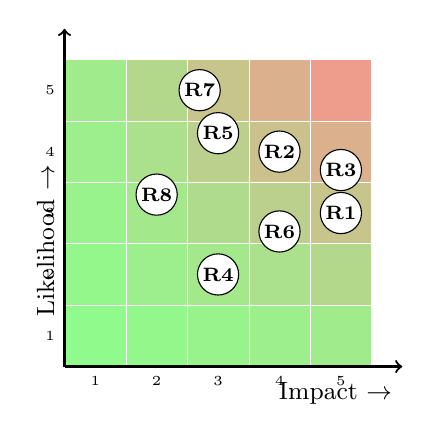
\begin{tikzpicture}[scale=0.78]
\foreach \x in {1,...,5} \foreach \y in {1,...,5} {
  \pgfmathsetmacro\s{(\x*\y)/25*85}
  \fill[red!\s!green!45] (\x-1,\y-1) rectangle (\x,\y);
  \draw[white, very thin] (\x-1,\y-1) rectangle (\x,\y);
}
\draw[->, thick] (0,0) -- (5.5,0) node[below left, yshift=-2pt]{\small Impact $\rightarrow$};
\draw[->, thick] (0,0) -- (0,5.5) node[above left, rotate=90, xshift=-1.6cm]{\small Likelihood $\rightarrow$};
\foreach \x in {1,...,5} \node[below, font=\tiny] at (\x-0.5,0) {\x};
\foreach \y in {1,...,5} \node[left, font=\tiny] at (0,\y-0.5) {\y};
\node[draw, circle, fill=white, inner sep=1pt, font=\scriptsize\bfseries] at (4.5,2.5) {R1};
\node[draw, circle, fill=white, inner sep=1pt, font=\scriptsize\bfseries] at (3.5,3.5) {R2};
\node[draw, circle, fill=white, inner sep=1pt, font=\scriptsize\bfseries] at (4.5,3.2) {R3};
\node[draw, circle, fill=white, inner sep=1pt, font=\scriptsize\bfseries] at (2.5,1.5) {R4};
\node[draw, circle, fill=white, inner sep=1pt, font=\scriptsize\bfseries] at (2.5,3.8) {R5};
\node[draw, circle, fill=white, inner sep=1pt, font=\scriptsize\bfseries] at (3.5,2.2) {R6};
\node[draw, circle, fill=white, inner sep=1pt, font=\scriptsize\bfseries] at (2.2,4.5) {R7};
\node[draw, circle, fill=white, inner sep=1pt, font=\scriptsize\bfseries] at (1.5,2.8) {R8};
\end{tikzpicture}
\caption{Risk matrix (post-mitigation assessment). The residual heavyweights are strategic, not technical: R3 (bus factor / no external users) and R2 (shared-host fragility). The technical risks that materialised (R1, R5, R6, R8) were each contained by the project's own instrumentation-first doctrine.}
\label{fig:riskmatrix}
\end{figure}

\subsection{What the materialised risks taught}

\textbf{R1 (cache correctness)} produced the project's defining management lesson. The cache's internal counters reported success while the measured cold hit rate was 0.4\,\% \emph{and} restores could break builds. The response was not a hotfix but a doctrine: instrument first (per-unit HIT/LOOKUPMISS/APPLYFAIL tracing), fix the key instability layer by layer, and ship a conservative default (populate-only) until restore can be proven safe against the recorded failure history. \textbf{R5 (build contention)} was an organisational failure mode --- multiple agents thrashing one build directory --- fixed structurally with atomic lane claims rather than behaviourally with pleas for coordination. \textbf{R8 (vandalised TeX binaries)} was discovered \emph{during the production of the project's own whitepaper}: two engine binaries had been silently overwritten by a stray shell redirect weeks earlier. It is the perfect miniature of the project's thesis --- unverified infrastructure rots silently; content-addressed identity is what makes rot detectable.

\section{Methodology: VarFlow Against the Textbook}
\label{sec:method}

The project's written methodology, VarFlow, maps cleanly onto --- and deliberately diverges from --- the agile canon of the HA(it.) curriculum:

\begin{table}[h]
\centering
\small
\begin{tabular}{@{}p{4.2cm}p{4.6cm}p{5.6cm}@{}}
\toprule
\textbf{Textbook construct} & \textbf{VarFlow equivalent} & \textbf{Divergence} \\
\midrule
Product backlog & Lane bounties on the swarm bus & Pull-based; no owner assigns work \\
Sprint / iteration & Ladder rung $\rightarrow$ release & Scope is a \emph{capability}, not a time-box \\
Definition of done & Measurement gate + settlement & Must be executable or recomputable \\
Daily stand-up & Bus messages (718 recorded) & Asynchronous, fully journaled \\
Retrospective & Honest checklist (``what is still pretend?'') & Runs \emph{before} claiming, not after \\
Steering committee & Arbiter model + human ratifier & Escalation is a model consultation \\
Team velocity & Settlement journal (716 tasks, 366 QUG) & Paid in internal work credits \\
\bottomrule
\end{tabular}
\caption{VarFlow vs.\ the agile textbook. The consistent theme: ceremonies are replaced by journals, and status is replaced by proof.}
\label{tab:varflow}
\end{table}

Two features deserve emphasis. First, the \textbf{four-question honesty checklist} (measurement gate? still pretend? composition edges? rollback path?) is a pre-commitment device: a lane that cannot answer all four is not ready to claim, which front-loads the quality discussion that Scrum defers to review. Second, \textbf{adversarial cross-review between heterogeneous models} is the default for non-trivial changes, on the empirical observation --- repeatedly confirmed this cycle --- that different model families miss different bugs. The v0.34 aggregate-binding fix, its cross-triaged parser root cause, and the release cut itself were three different agents' verified work, coordinated entirely over the bus.

\section{Technical Achievement (Enhanced from the Whitepaper)}

This section carries the whitepaper's strongest material, strengthened with a figure the paper lacked, and framed for a mixed business/technical reader.

\subsection{The architecture in one picture}

\begin{figure}[h]
\centering
\begin{tikzpicture}[
  node distance=0.55cm and 0.7cm,
  box/.style={draw, rounded corners=2pt, align=center, font=\small, minimum height=0.95cm, inner xsep=6pt},
  own/.style={box, fill=accent!18, draw=accent!60!black},
  borrow/.style={box, fill=gray!15, draw=gray!60},
  side/.style={box, fill=gold!18, draw=gold!60!black, font=\scriptsize},
  arr/.style={->, thick}
]
\node[borrow] (rustc) {\texttt{rustc --emit=mir}\\ \scriptsize borrowed, pinned 1.93.1\\ \scriptsize type + borrow check};
\node[own, right=of rustc] (fe) {\texttt{flux-frontend}\\ \scriptsize parse\_mir $\rightarrow$ Flux IR\\ \scriptsize consts, monomorph.};
\node[own, right=of fe] (be) {\texttt{flux-backend}\\ \scriptsize IR $\rightarrow$ CLIF\\ \scriptsize Cranelift, verified};
\node[own, right=of be] (elf) {native ELF\\ \scriptsize \texttt{cc}/\texttt{mold} link};
\node[side, below=of fe] (cache) {\texttt{flux-cache}: BLAKE3 content-addressed build cache\\ populate by default, restore opt-in (safety before speed)};
\node[side, below=of be] (rev) {\texttt{flux-rev}: recomputable\\ release identity (BLAKE3)};
\draw[arr] (rustc) -- node[above, font=\tiny]{MIR text} (fe);
\draw[arr] (fe) -- (be);
\draw[arr] (be) -- (elf);
\draw[arr, dashed, gray] (cache.north) -- (fe.south);
\draw[arr, dashed, gray] (rev.north) -- (be.south);
\end{tikzpicture}
\caption{The contracted-frontend architecture. Grey is borrowed and carries the entire soundness burden; blue is owned (under 4{,}000 lines for the compiler core); gold is the provenance/caching sidecar. The seam is rustc's MIR: all safety analysis done, no codegen decisions made.}
\label{fig:arch}
\end{figure}

The strategic content of FIP-0001 (accepted 2026-06-26) is a \emph{make-or-buy decision}, in classic IT-management terms: the frontend --- roughly two-thirds of a Rust compiler's complexity and the seat of its safety guarantees --- is \emph{bought} (contracted from rustc at a pinned version), while codegen, caching, and provenance --- the differentiating value --- are \emph{made}. The buy side costs one operational dependency and the acceptance that memory-safety guarantees remain rustc's; the make side captured six shipped releases in eight days. The north-star option (owning the frontend) is preserved behind a measurable trigger rather than abandoned --- an embedded real option, kept cheap by five groundwork items (frozen IR spec, MIR-drift CI, a \texttt{Frontend} trait seam, a coupling audit, cached std rlibs).

\subsection{Evaluation results, consolidated}

\begin{table}[h]
\centering
\small
\resizebox{\textwidth}{!}{%
\begin{tabular}{@{}llll@{}}
\toprule
\textbf{Claim} & \textbf{Evidence} & \textbf{Kind} & \textbf{Where} \\
\midrule
Rungs 1--6 compile correctly & exit-value proofs (\texttt{pick((1,2),(3,4))}=34, \ldots) & executable & every release tag \\
Aggregate params bind correctly & disassembly: \texttt{xor rax,rax} $\rightarrow$ \texttt{mov rdx,rax} & disassembly & v0.34 cycle \\
Test suites green & flux-backend 43/43, flux-frontend 16/16 & test run & \texttt{flux\_combo} \\
Cache was broken & measured 0.4\,\% cold; trace HIT=0/37 & instrumentation & FIP-0002 \\
Cache key fix works & trace 0/37 $\rightarrow$ 14/35 on identical rebuild & instrumentation & v0.33 \\
Release identity recomputable & flux-rev \texttt{full:6f2eaff4\ldots} & recomputation & v0.34.0 \\
Swarm coordination works & 51 agents, 718 msgs, 716 settled, 0 collisions & journal & settlement log \\
Docs build through the toolchain & this report + the whitepaper & self-exhibit & flux-arxiv-latex \\
\bottomrule
\end{tabular}%
}
\caption{Consolidated evaluation. Each claim names its evidence \emph{kind} --- the project's rule is that a claim without an executable, recomputable, or journaled proof is ``still pretend.''}
\label{tab:eval}
\end{table}

\section{Business Case and SWOT}

Flux is pre-revenue by construction; the honest business case is an \emph{asset-building} one. Costs are concentrated and modest: one build server, model-API consumption for the swarm, and the maintainer's direction time. Against that, the project has produced three assets with independent option value: (1) the \textbf{compiler}, a working demonstration that contracted-frontend self-hosting works, with a defensible honest-measurement story; (2) the \textbf{agent-native platform} --- the swarm bus, combo tools, and settlement journal are a working answer to ``how do multiple AI agents safely ship one codebase,'' a question the industry is actively buying answers to; (3) the \textbf{provenance stack}, aligned with a regulatory tailwind (software supply-chain verification). The internal QUG credit economy (366 QUG settled across 716 tasks) is today an accounting device, not revenue --- but it is also a rehearsal for pricing agent labour, and the journal it produces is exactly the audit trail a future commercial deployment would need.

\begin{figure}[h]
\centering
\begin{tikzpicture}[
  q/.style={draw, rounded corners=3pt, text width=0.44\textwidth, inner sep=7pt, font=\small, align=left, minimum height=3.3cm}
]
\node[q, fill=okgreen!12, draw=okgreen!60!black] (s) at (0,0)
  {\textbf{Strengths}\\[2pt] contracted-frontend architecture (fast, sound); working multi-agent delivery system with journaled proof; verify-don't-trust provenance; 6 releases / 8 days demonstrated};
\node[q, fill=risk!10, draw=risk!60!black, right=0.5cm of s] (w)
  {\textbf{Weaknesses}\\[2pt] single operator, zero external users; 143-crate sprawl vs.\ $\sim$15-crate core; cache safe but not yet fast (Phase 2 unshipped); traits rung still ahead};
\node[q, fill=accent!12, draw=accent!60!black, below=0.5cm of s] (o)
  {\textbf{Opportunities}\\[2pt] industry demand for safe agent-swarm engineering; supply-chain verification regulation; agent-labour pricing (QUG rehearsal); FCX native-UI niche (3.6\,MB, no Electron)};
\node[q, fill=gold!15, draw=gold!60!black, right=0.5cm of o] (t)
  {\textbf{Threats}\\[2pt] rustc-MIR drift (controlled but real); model-API cost and availability; shared-host fragility (R2, R8); attention: the operator is the scarcest resource};
\end{tikzpicture}
\caption{SWOT. The decisive quadrant is Opportunities vs.\ the single-operator Weakness: the assets are real, but converting them requires either external adopters or deliberate productisation of one core slice.}
\label{fig:swot}
\end{figure}

\section{Conclusion and Perspectives}

Judged as a project, Flux exhibits an unusual and instructive profile. \textbf{Planning}: the phase structure was emergent but disciplined --- capability-scoped sprints (ladder rungs) rather than time-boxes, with milestones that carry their own proofs (Table~\ref{tab:milestones}). \textbf{Risk}: four of eight register entries materialised, and each was contained by the project's instrumentation-first doctrine; the residual top risks are strategic (bus factor, no external users), not technical. \textbf{Value}: the business case is an asset case --- compiler, platform, provenance --- with the swarm-coordination system as the most externally marketable of the three.

The perspectives follow directly from the register and the ledger. Near-term (P7): the FIP-0001 groundwork items and FIP-0002 Phase 2, whichever proves first --- both reduce the project's largest technical debts. Mid-term (P8): the 0.36.x hardening release, which converts a 20/22-closed security audit into a shippable trust claim. Strategic: address R3 --- either by attracting external adopters to one polished slice (the swarm platform is the obvious candidate) or by explicitly accepting Flux as a research vehicle and pricing it as such. The Gantt chart's ``Planned'' group is short on purpose: in a project whose method is \emph{two minds propose, the build disposes}, plans beyond one phase are hypotheses, and the ledger --- git, flux-rev, and the settlement journal --- will keep the score.
